% Created 2026-03-07 Sat 13:07
% Intended LaTeX compiler: pdflatex
\documentclass[11pt, letterpaper]{article}
\usepackage[utf8]{inputenc}
\usepackage[T1]{fontenc}
\usepackage{graphicx}
\usepackage{longtable}
\usepackage{wrapfig}
\usepackage{rotating}
\usepackage[normalem]{ulem}
\usepackage{amsmath}
\usepackage{amssymb}
\usepackage{capt-of}
\usepackage{hyperref}
\usepackage[margin=2.5cm]{geometry}      % Márgenes decentes
\usepackage[utf8]{inputenc}
\usepackage{palatino}                   % Tipografía elegante
\usepackage{xcolor}                     % Colores personalizados
\author{mrtaichi}
\date{\today}
\title{Writeup - Fruityloops EchoCTF}
\hypersetup{
 pdfauthor={mrtaichi},
 pdftitle={Writeup - Fruityloops EchoCTF},
 pdfkeywords={},
 pdfsubject={},
 pdfcreator={Emacs 30.2 (Org mode 9.7.29)}, 
 pdflang={English}}
\begin{document}

\maketitle
\setcounter{tocdepth}{2}
\tableofcontents

\begin{center}
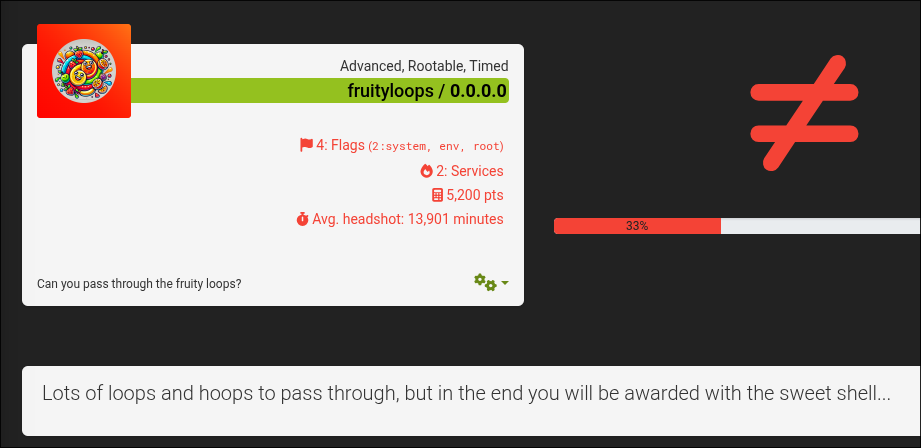
\includegraphics[width=.9\linewidth]{./1.png}
\end{center}
\section{Información General}
\label{sec:org42b10cf}


\begin{itemize}
\item \textbf{\textbf{Nombre de la Máquina}}: fruityloops
\item \textbf{\textbf{Plataforma}}: echoCTF
\item \textbf{\textbf{Dificultad}}: Medio
\item \textbf{\textbf{Sistema Operativo}}: Linux
\item \textbf{\textbf{Fecha}}: 2026-06-03
\item \textbf{\textbf{Autor}}: mrtaichi
\end{itemize}
\section{Descripción de la máquina}
\label{sec:org6163d3d}
Lots of loops and hoops to pass through, but in the end you will be awarded with the sweet shell\ldots{}
\section{Enumeración}
\label{sec:orgd3c8bc6}

\subsection{Escaneo Inicial}
\label{sec:org46d5fb9}

Inmediatamente probamos entrar por http a la máquina a ver que nos encontramos. De esta forma, encontramos directamente una página web a la cual por más que le rasquemos no vamos a encontrar mucho. Esto porque es simplemente una plantilla HTML que no nos da nada.

\begin{center}
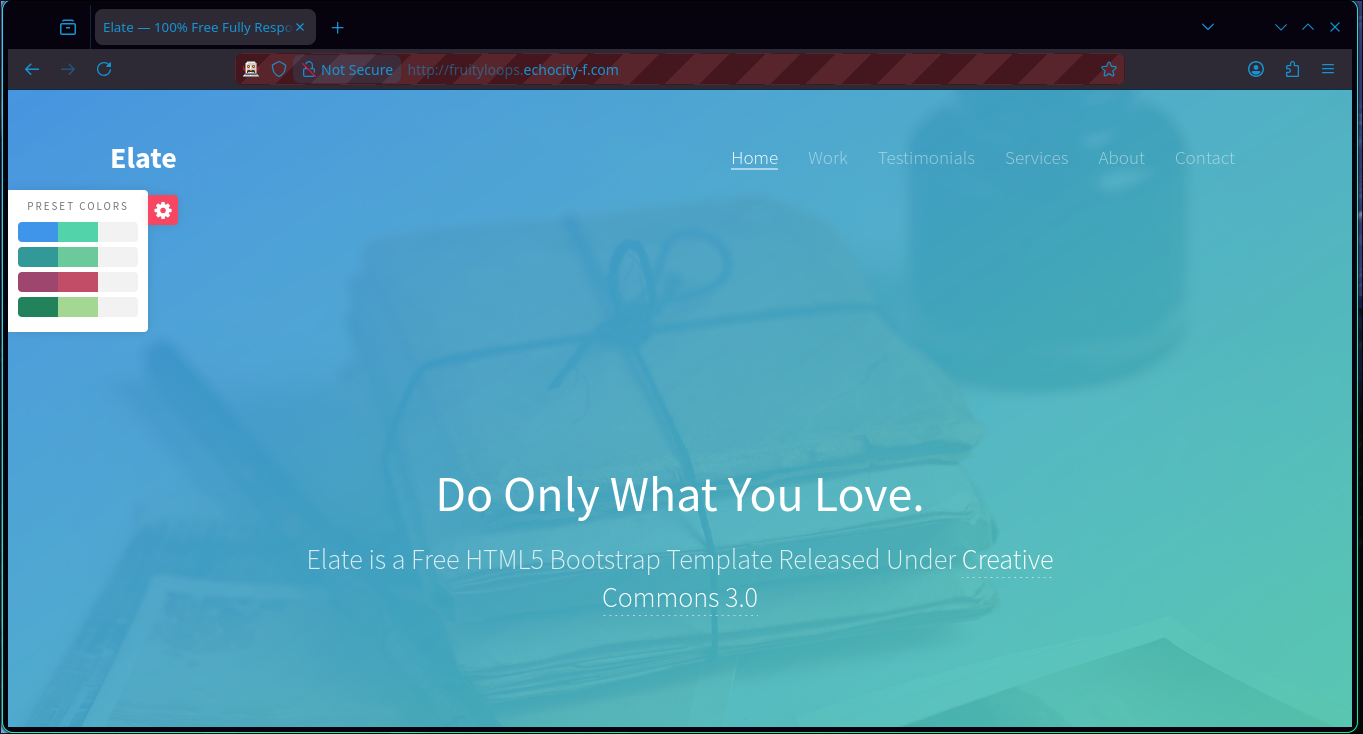
\includegraphics[width=.9\linewidth]{./2.png}
\end{center}
\subsection{Análisis de Servicios}
\label{sec:orgcb79d94}

Ya tenemos 1/2 servicios identificados. El otro es un SSH que identificamos cuando corremos un nmap sobre la máquina.

De una vez también hacemos un dirsearch para ver qué nos podemos topar.

\begin{center}
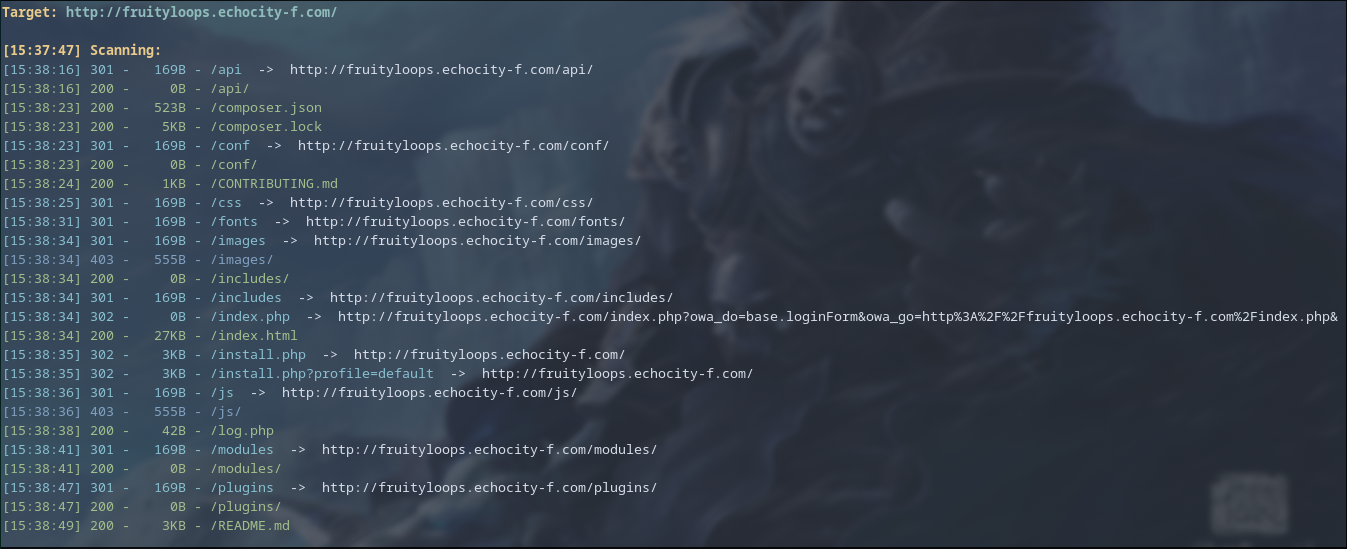
\includegraphics[width=.9\linewidth]{./3.png}
\end{center}

En este dirsearch nos podemos topar varias cosillas ya bastante interesantes. Pero lo más interesante y a donde debemos de dirigir nuestra atención son dos cosas:

\begin{itemize}
\item Tenemos un index.php, generalmente un index.php nos da más lógica explotable que el index.html al que tenemos acceso.

\item Tenemos un README.md
\end{itemize}

En el README encontramos la descripción de un servicio llamado Open Web Analytics, y de hecho el index.php es el admin panel del mismo.

\begin{center}
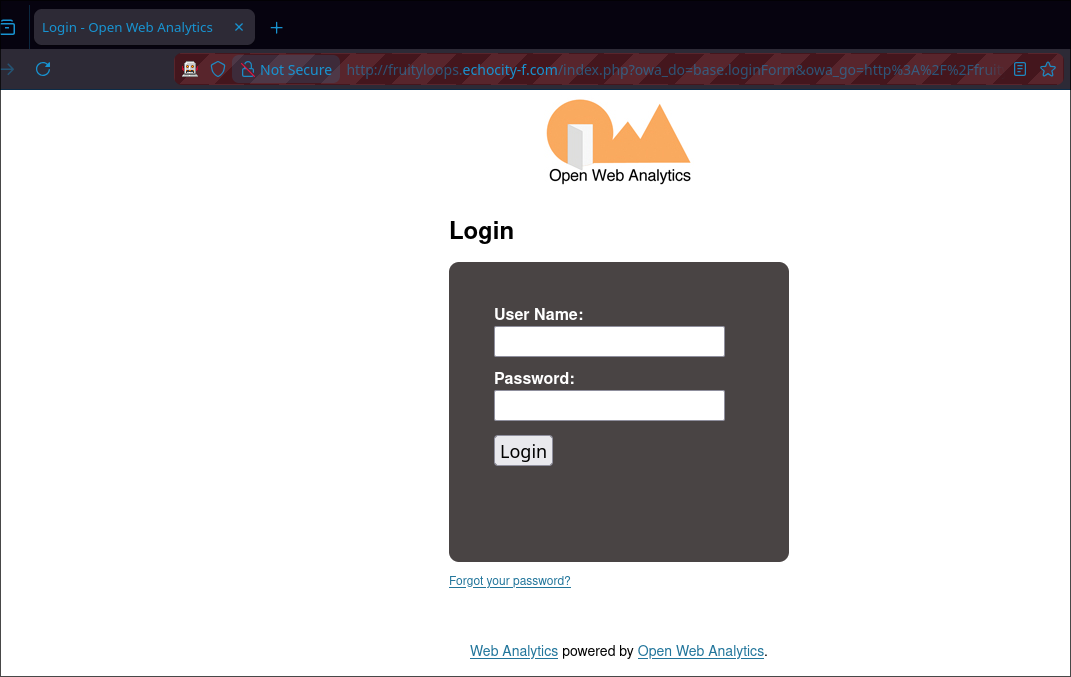
\includegraphics[width=.9\linewidth]{./4.png}
\end{center}
\section{Explotación}
\label{sec:orgb586dcb}

\subsection{Busqueda de vulnerabilidades}
\label{sec:org66ecb50}

Si googleamos Open Web Analytics, nos encontramos directamente con una vulnerabilidad relacionada con Remote Code Execution. Esto nos sirve.

\begin{center}
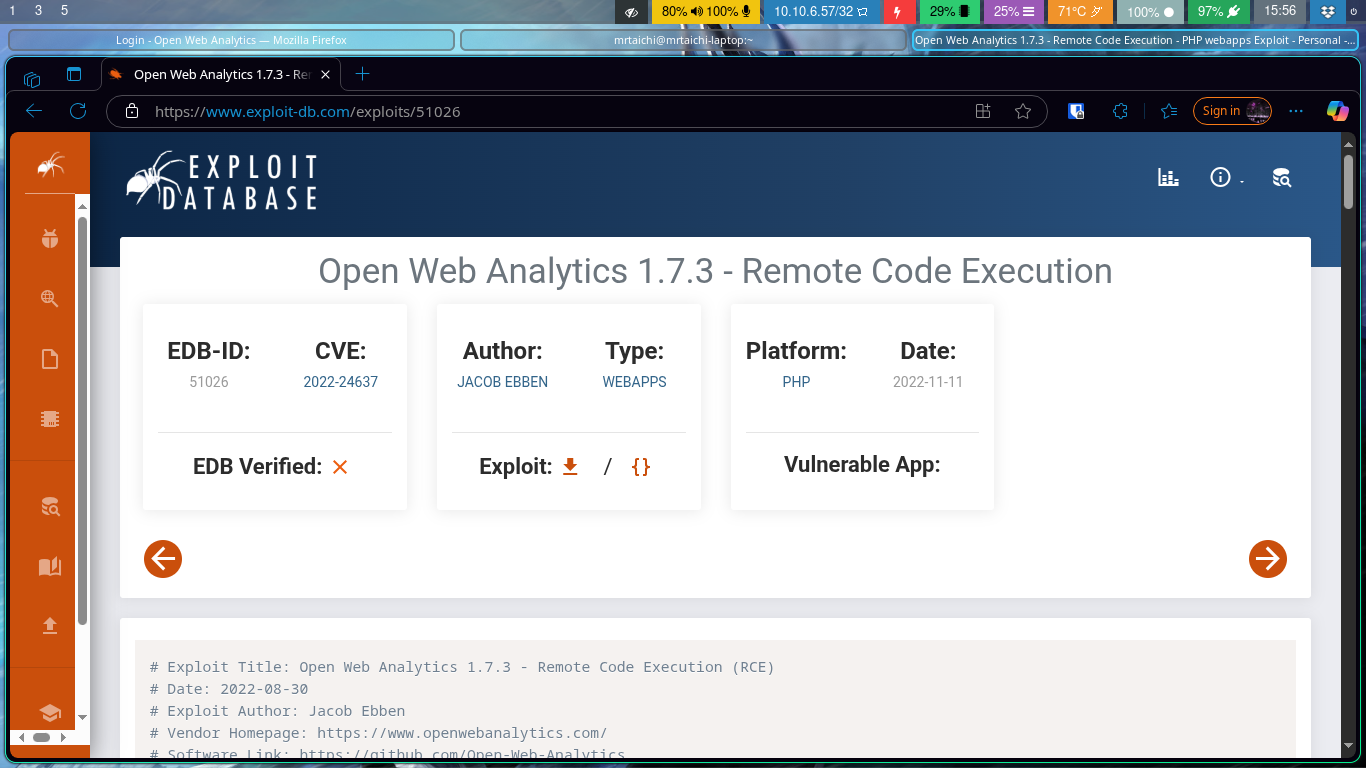
\includegraphics[width=.9\linewidth]{./5.png}
\end{center}
\subsection{Intentos de explotaciones}
\label{sec:orgede8076}
Si intentamos correr el script directamente vamos a tumbar la máquina, entonces debemos de realizar algunos cambios.

El primero y el más directo es cambiar el payload que crea la reverse shell, esto porque utiliza sockets; y las máquinas de echoCTF no admiten el uso de sockets para levantar revshells. Así que usemos netcat para esto.

\begin{center}
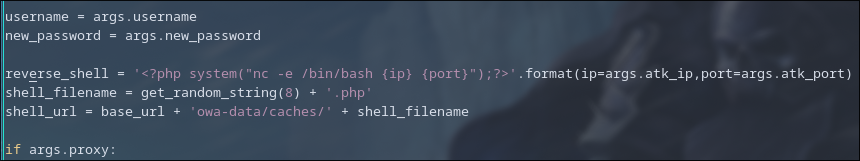
\includegraphics[width=.9\linewidth]{./6.png}
\end{center}

En la linea 100 cambiamos el payload para que sea un php que use ese comando simplemente. Con esto, el payload puede funcionar correctamente.

El segundo cambio que vamos a realizar es relacionado a la forma en que funciona la vulnerabilidad:

La vulnerabilidad se sirve de crear un archivo log el cual puede ser un php interpretable. El problema con el exploit es que asume que los logs se crean en \emph{var/www/html/owa/owa-data/caches}. Esto no es correcto en el contexto de esta máquina. Para ver la ruta real, debemos de bypassear el panel de admin con las primeras partes del exploit y meternos a manita para ver la ruta real.

Para esto, comentamos todo después de la linea 204:

\begin{center}
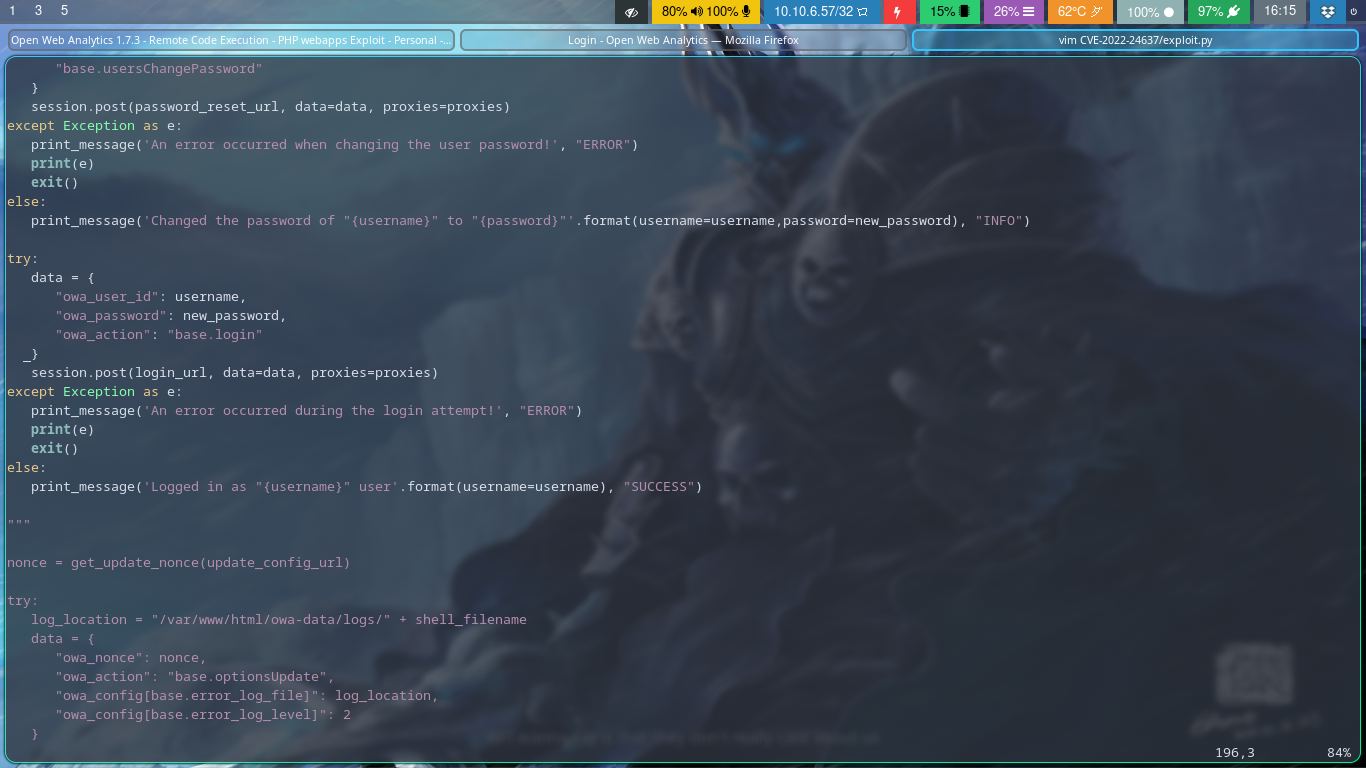
\includegraphics[width=.9\linewidth]{./7.png}
\end{center}

Con esto corremos el script solamente para cambiar la contraseña del admin y poder acceder

\begin{center}
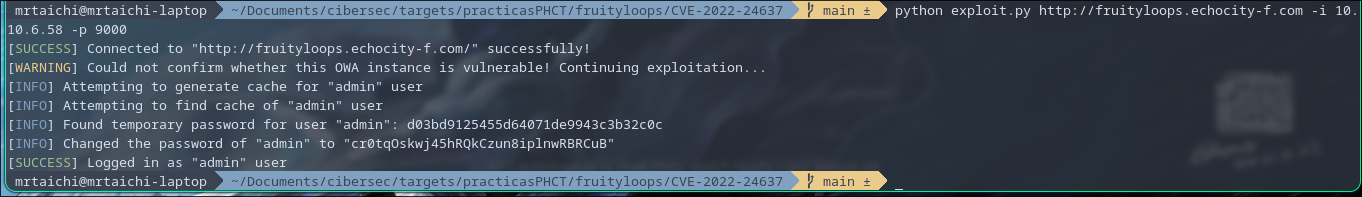
\includegraphics[width=.9\linewidth]{./8.png}
\end{center}
\subsection{Explotación}
\label{sec:orgd1e6cb7}
Al entrar a la sección de Settings -> Main Configuration nos encontramos bajo la sección de eventos la ruta real a la que vamos a guardar los logs, la cual es /var/www/html/owa-data/logs

\begin{center}
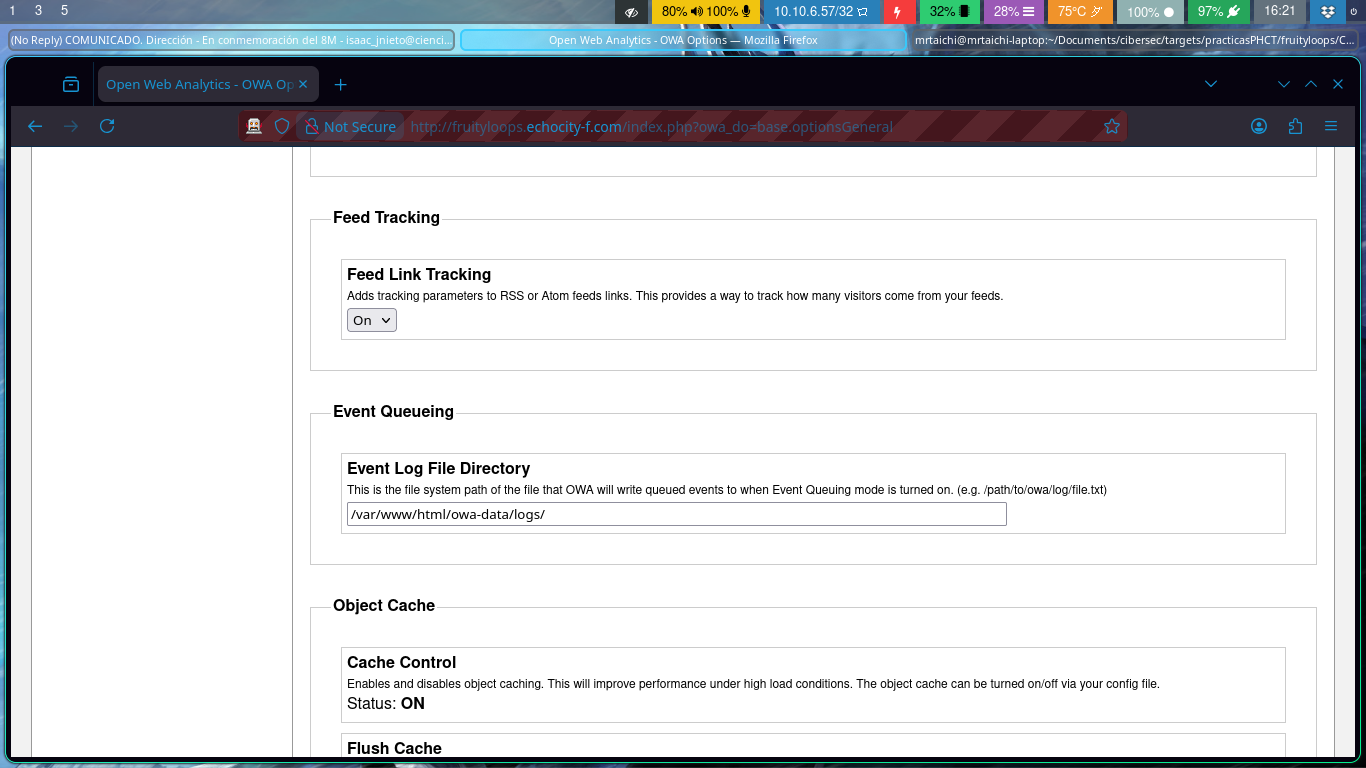
\includegraphics[width=.9\linewidth]{./9.png}
\end{center}

Es a esta ruta a la que debe apuntar nuestro script. La usamos en dos ámbitos: para guardar el log y para activarlo.

Para corregir el script, corregimos esta ruta en dos lugares clave:

En la variable log\textsubscript{location}, alrededor de la linea 209

Y en la variable shell\textsubscript{url}, alrededor de la línea 102:

\begin{center}
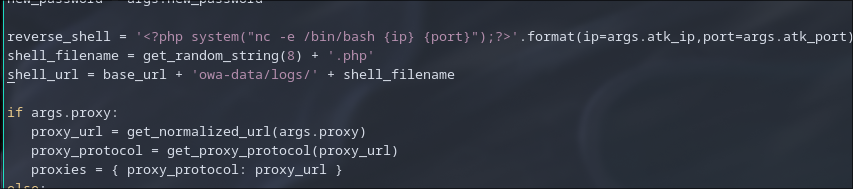
\includegraphics[width=.9\linewidth]{./10.png}
\end{center}

Con estos cambios, podemos descomentar la última sección del script, poner a nuestro manejador de revshells predilecto a la escucha y correr el script.

\begin{center}
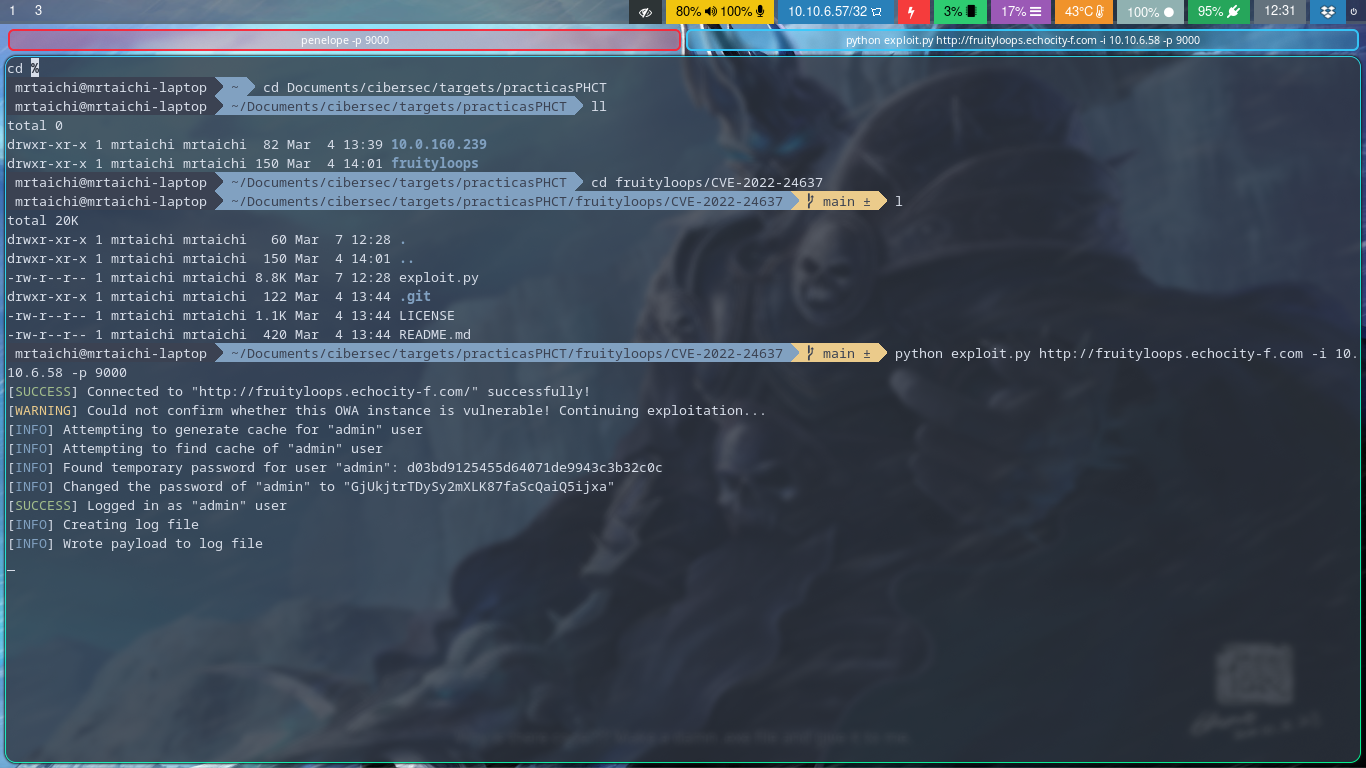
\includegraphics[width=.9\linewidth]{./11.png}
\end{center}

\begin{center}
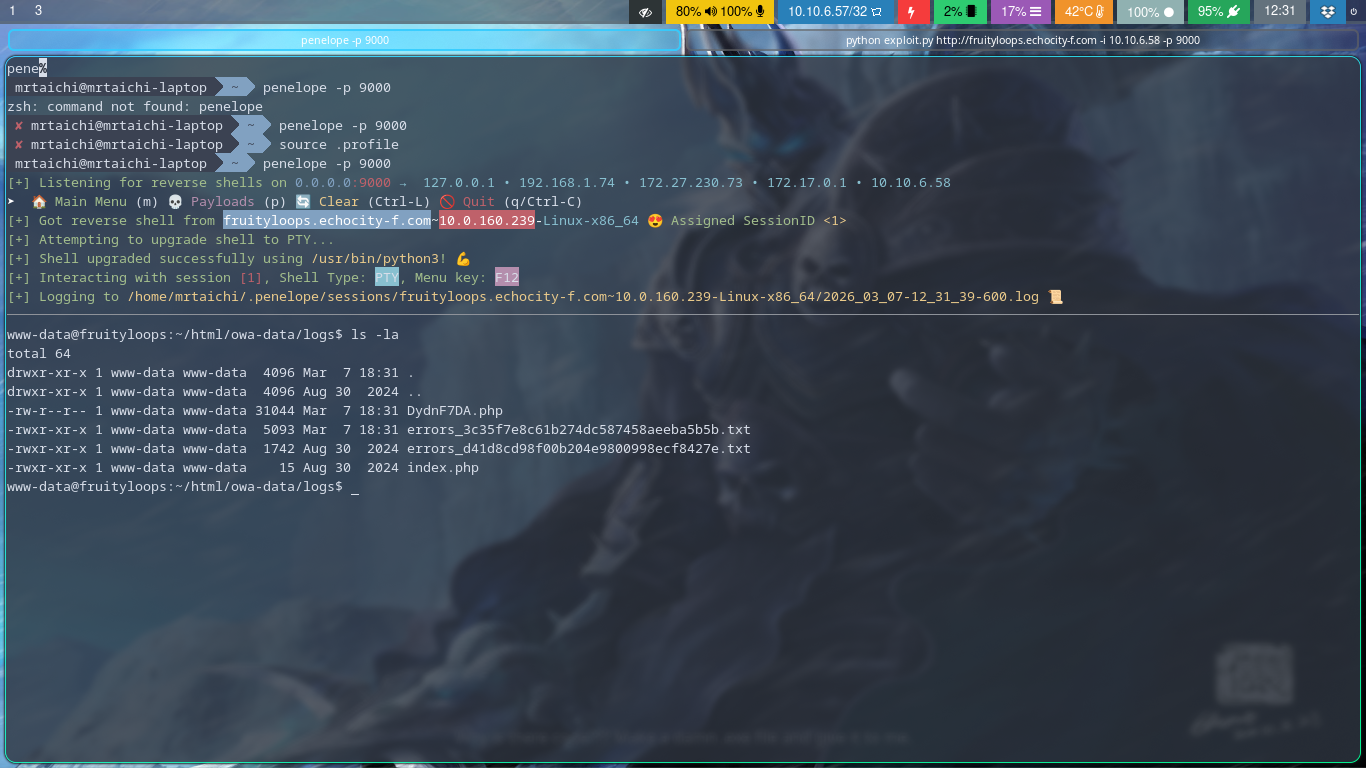
\includegraphics[width=.9\linewidth]{./12.png}
\end{center}

Y estamos dentro
\section{Escalación de Privilegios}
\label{sec:orged42ca5}

\subsection{Análisis}
\label{sec:orga24da73}

Entramos a la máquina como el usuario www-data (típico de máquinas de EchoCTF).

Mi regla de dedo es siempre correr sudo -l antes que nada, para ver si podemos correr algún binario con permisos de root ya desde ahora. Y efectivamente, tenemos un script en Javascript que podemos correr con sudo sin contraseña

\begin{center}
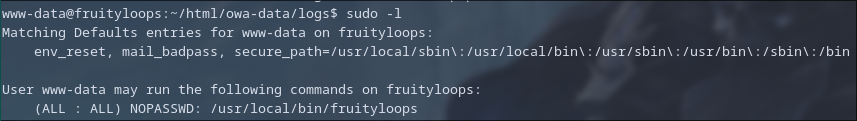
\includegraphics[width=.9\linewidth]{./13.png}
\end{center}

El cual me huele a un Prototype Pollution de manual.

Y efectivamente, si googleamos la única biblioteca que utiliza este script (apphp/object-resolver), podemos encontrar una vulnerabilidad de Prototype Pollution, cuyo ejemplo es extremadamente parecido al código que tenemos en el script.

\url{https://gist.github.com/mestrtee/c90189f3d8480a5f267395ec40701373}
\subsection{Explotación}
\label{sec:org959c9a3}

El \textbf{\textbf{Prototype Pollution}} ocurre cuando una aplicación permite a un atacante modificar el prototipo de un objeto base (normalmente `Object.prototype`). En JavaScript, casi todos los objetos heredan propiedades de este prototipo.

En el código de `/usr/local/bin/fruityloops`, observamos lo siguiente:

\begin{enumerate}
\item Se define un objeto vacío `var authentication = \{\}`.

\item Se utiliza la función vulnerable `lib.setNestedProperty(\{\}, args[0], true)`.

\item Se verifica si `authentication.success \texttt{=} true`.
\end{enumerate}

Normalmente, `authentication.success` sería `undefined` porque el objeto está vacío. Sin embargo, si logramos ``contaminar'' el prototipo global de los objetos, cualquier objeto nuevo (incluyendo `authentication`) heredará la propiedad que nosotros definamos.

La biblioteca `@apphp/object-resolver` no sanitiza la llave que se le pasa en el primer argumento. Si enviamos el string `\_\textsubscript{proto}\_\textsubscript{.success}`, la función no modificará el objeto temporal `\{\}`, sino que subirá en la jerarquía hasta el objeto raíz y le asignará el valor `true` a la propiedad `success`.

El script intenta ejecutar un binario en `/tmp/pwned`. Como somos `www-data`, tenemos permisos de escritura en `/tmp`, así que creamos un script que nos devuelva una shell con privilegios:

\begin{verbatim}
# Creamos el archivo que ejecutará el script de Node
echo -e '#!/bin/bash\nchmod +s /bin/bash' > /tmp/pwned

# Le damos permisos de ejecución
chmod +x /tmp/pwned

\end{verbatim}

Ahora ejecutamos el binario con `sudo`. Al pasarle el string de contaminación como argumento, el `if` se volverá verdadero y el proceso ejecutará nuestro archivo en `/tmp` con los permisos de `sudo` (root).

\begin{verbatim}
sudo /usr/local/bin/fruityloops "__proto__.success"
\end{verbatim}

¡Y listo! Al ejecutarse, le damos SUID a /bin/bash y con eso, al ejecutarla con -p, podemos escalar a root.

\begin{center}
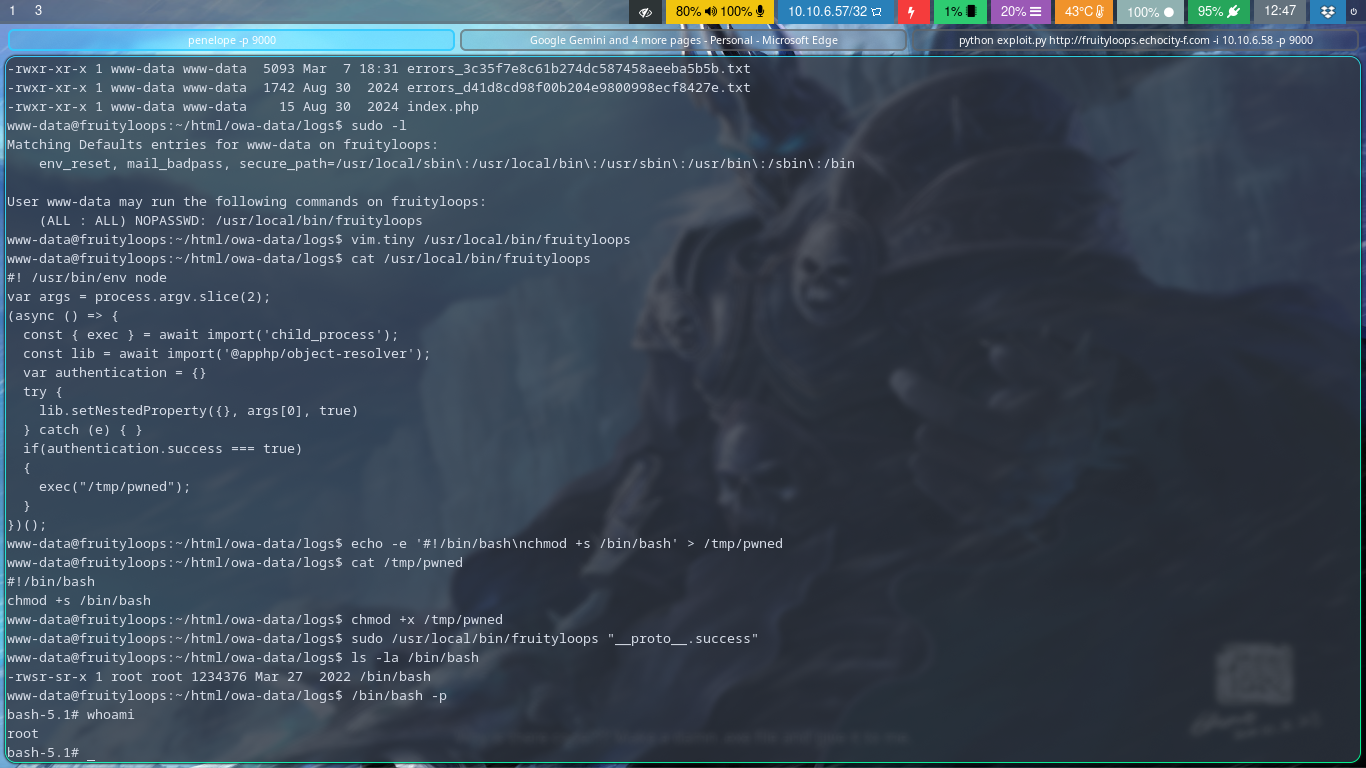
\includegraphics[width=.9\linewidth]{./14.png}
\end{center}

Una vez como root, solo queda buscar las flags.

\begin{itemize}
\item Dos de system: las de /etc/shadow y /etc/passwd
\item La de env, en /proc/1/environ
\item La de root, el archivo en /root
\end{itemize}

\textbf{\textbf{HEADSHOT}}
\end{document}
